\begin{figure*}
  \centering
    \begin{subfigure}[c]{0.05\textwidth}
    ~
  \end{subfigure}
  % 
  \begin{subfigure}[c]{0.45\textwidth}
    \centering
    ~~\textbf{Mild plate effects}
  \end{subfigure}
  % 
  \begin{subfigure}[c]{0.45\textwidth}
    \centering
    ~~\textbf{Strong plate effects}
  \end{subfigure}

  \begin{subfigure}[c]{0.05\textwidth}
    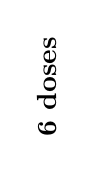
\begin{tikzpicture}
      \node[rotate=90] {\textbf{6 doses}};  
    \end{tikzpicture}
  \end{subfigure}  
  %
  \begin{subfigure}[c]{0.45\textwidth}
    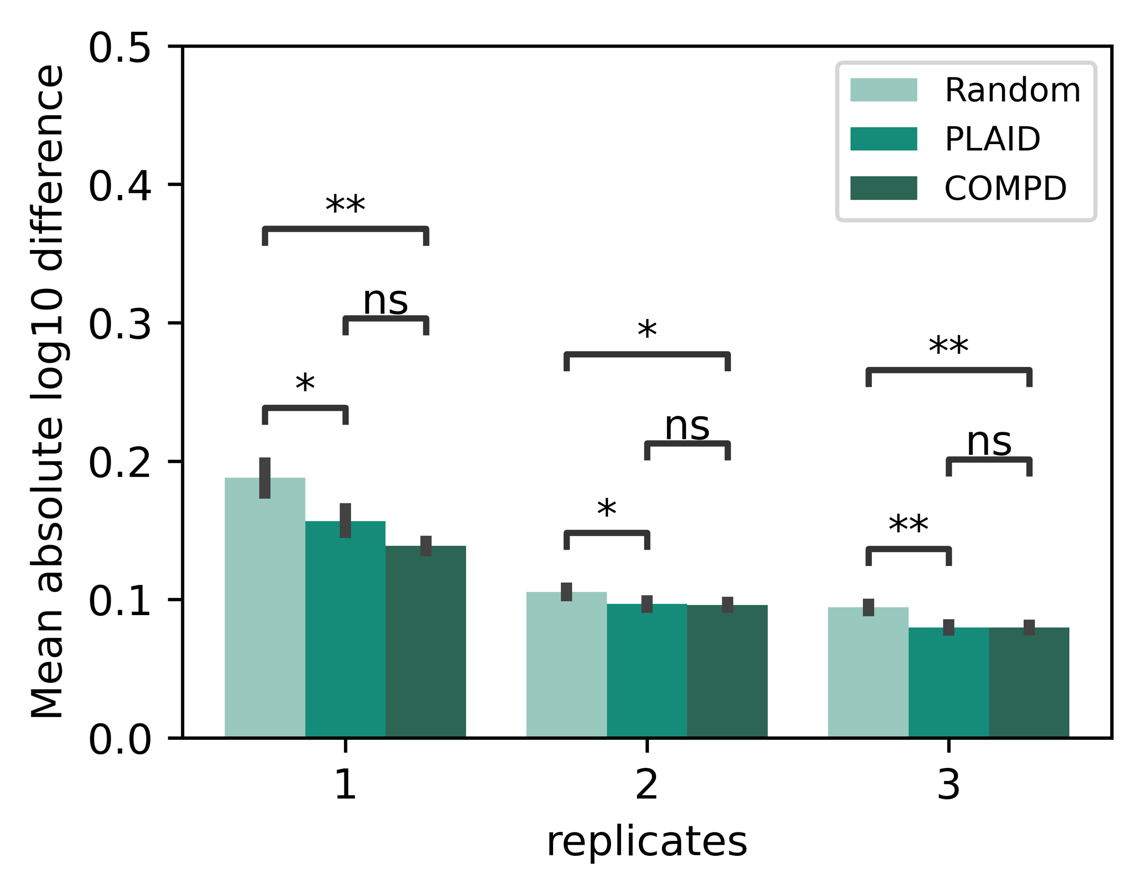
\includegraphics[width=\textwidth]{figures/dose-response-relic50-1-2-3-6doses-dil18-half-columns-neg-controls-0.2.png}
    %\caption{relic50 6doses-dil8-bowl-0.055}
    % \label{fig:tem}
  \end{subfigure}
  %
  \begin{subfigure}[c]{0.45\textwidth}
    \centering
    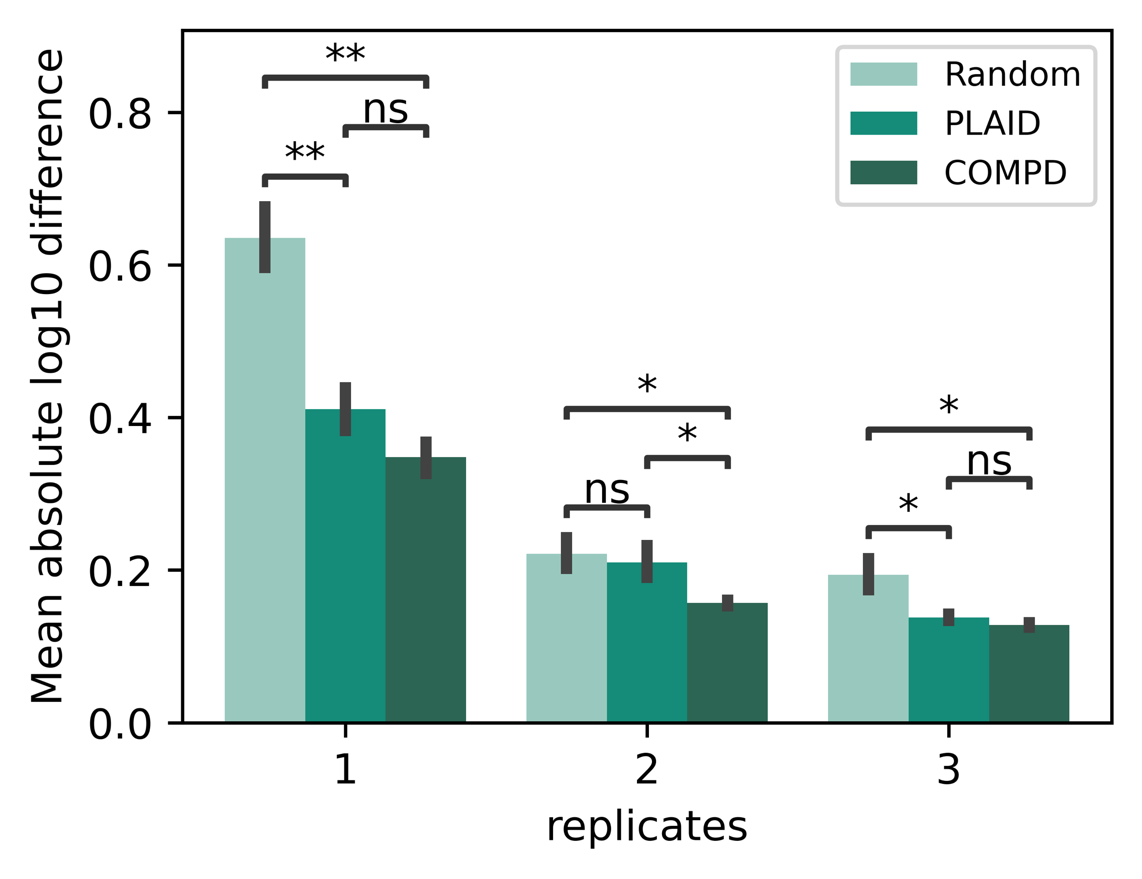
\includegraphics[width=\textwidth]{figures/dose-response-relic50-1-2-3-6doses-dil18-half-columns-neg-controls-0.4.png}
    %\caption{relic50 6doses-dil18-bowl-0.085}
    % \label{fig:tem}
  \end{subfigure}

    \begin{subfigure}[c]{0.05\textwidth}
    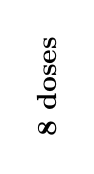
\begin{tikzpicture}
      \node[rotate=90] {\textbf{8 doses}};  
    \end{tikzpicture}
  \end{subfigure}  
  %
  \begin{subfigure}[c]{0.45\textwidth}
    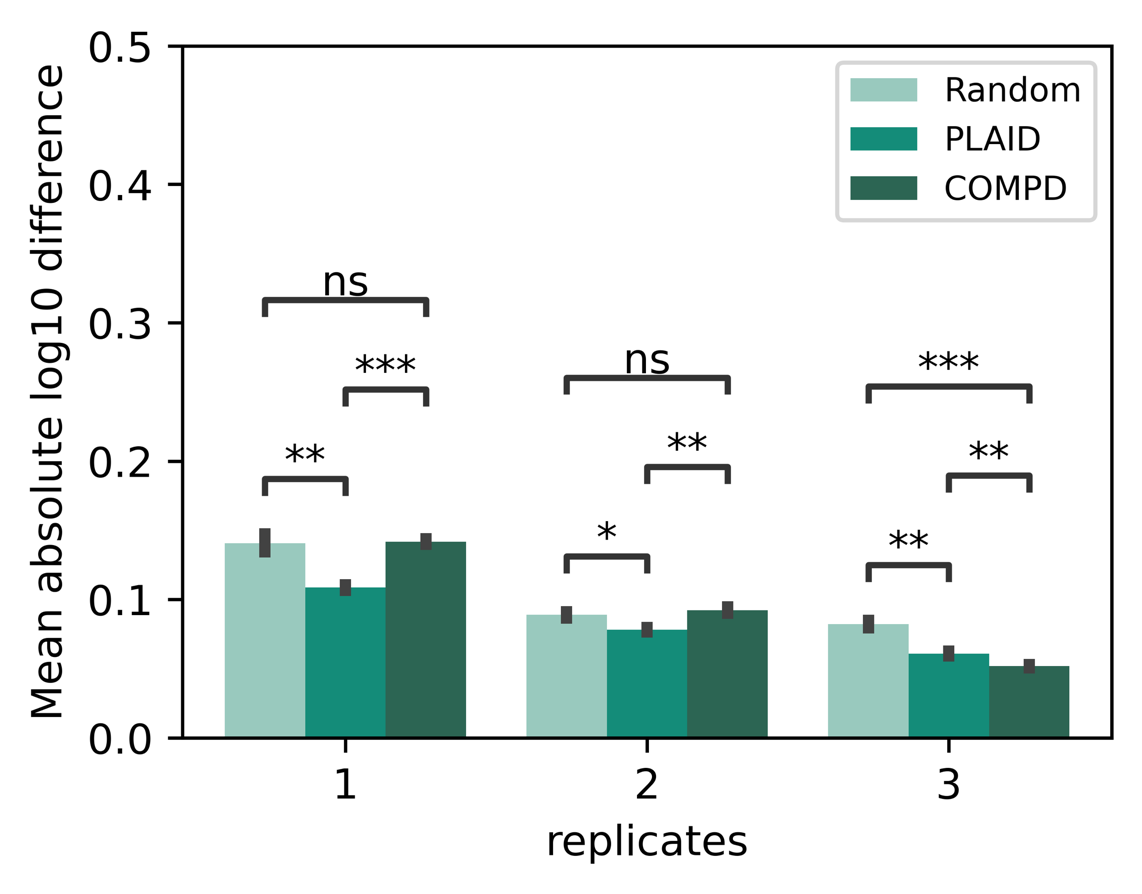
\includegraphics[width=\textwidth]{figures/dose-response-relic50-1-2-3-8doses-dil8-half-columns-neg-controls-0.2.png}
    %\caption{relic50 8doses-dil8-bowl-0.055}
    % \label{fig:tem}
  \end{subfigure} 
  %
  \begin{subfigure}[c]{0.45\textwidth}
    \centering
    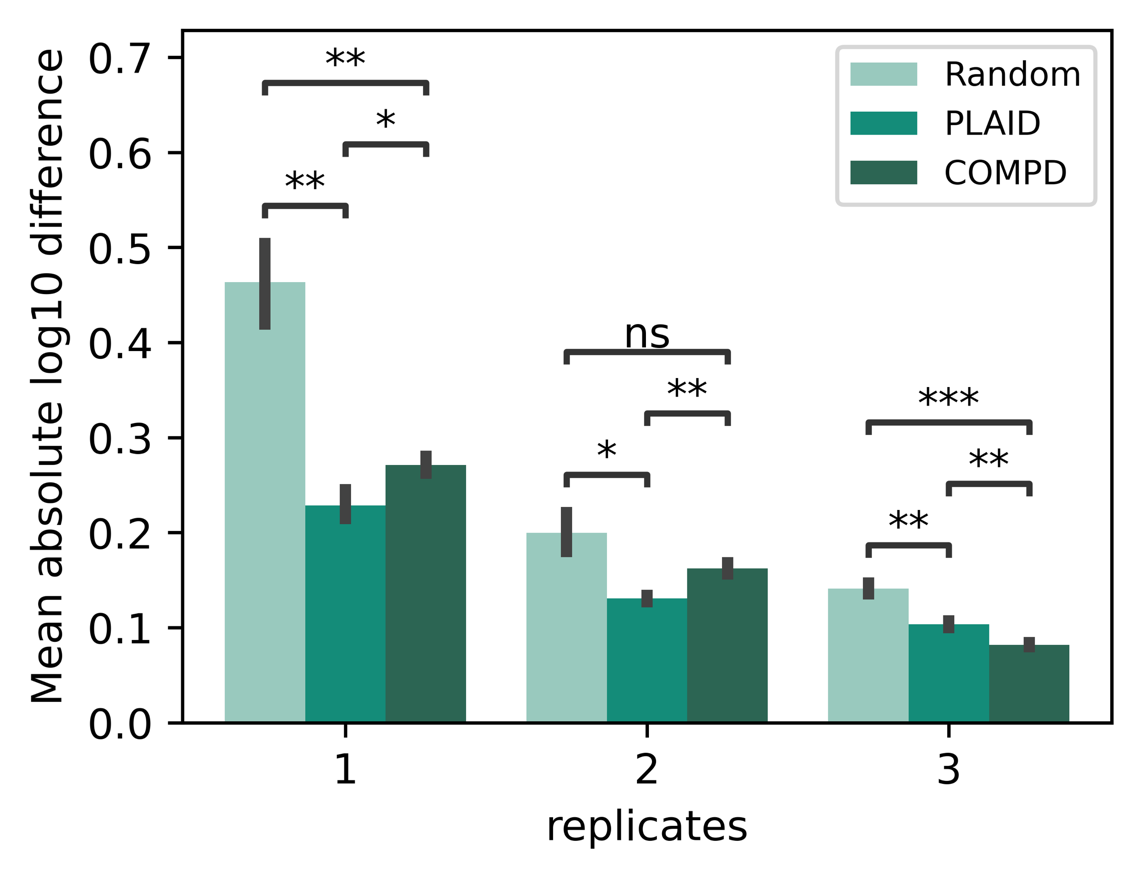
\includegraphics[width=\textwidth]{figures/dose-response-relic50-1-2-3-8doses-dil8-half-columns-neg-controls-0.4.png}
    %\caption{relic50 8doses-dil8-bowl-0.085}
    % \label{fig:tem}
  \end{subfigure}

    \begin{subfigure}[c]{0.05\textwidth}
    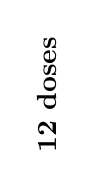
\begin{tikzpicture}
      \node[rotate=90] {\textbf{12 doses}};  
    \end{tikzpicture}
  \end{subfigure}  
  %
   \begin{subfigure}[c]{0.45\textwidth}
    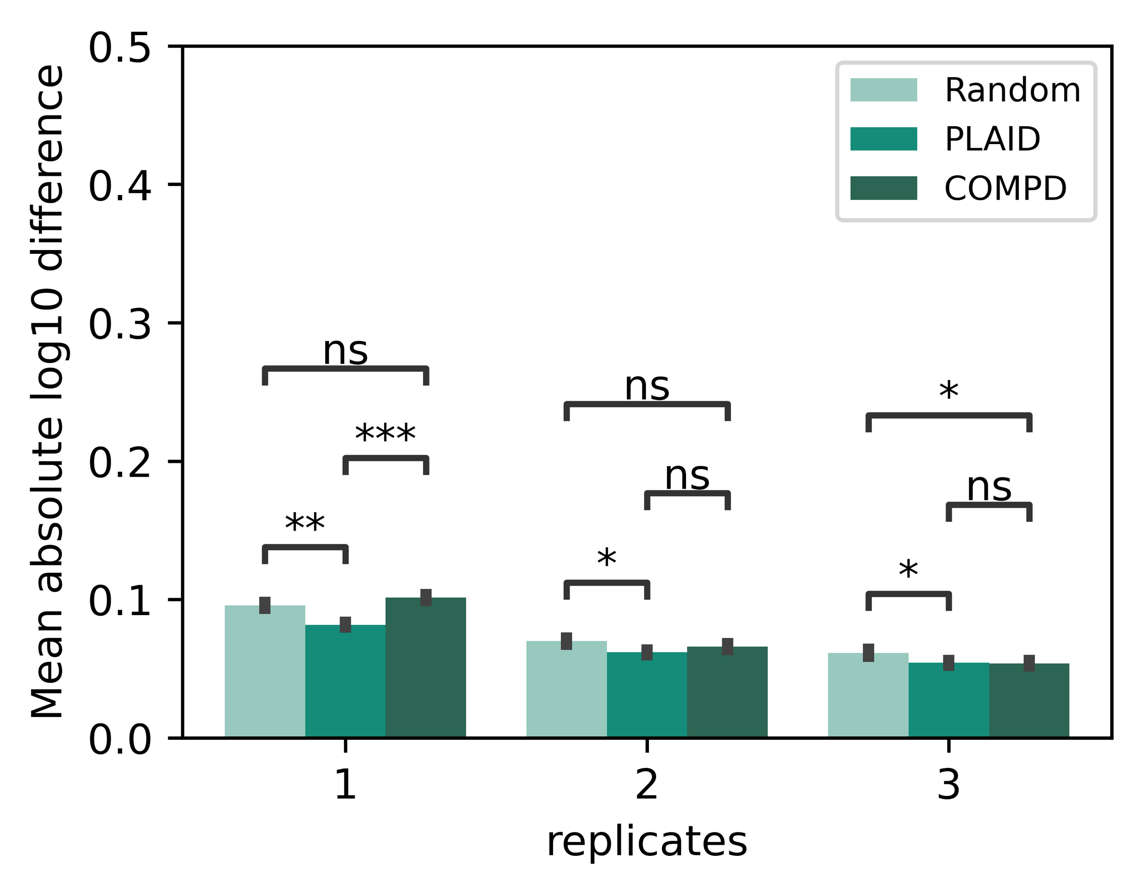
\includegraphics[width=\textwidth]{figures/dose-response-relic50-1-2-3-12doses-dil4-half-columns-neg-controls-0.2.png}
    %\caption{relic50 12doses-dil4-bowl-0.055}
    % \label{fig:tem}
  \end{subfigure} 
  %
  \begin{subfigure}[c]{0.45\textwidth}
    \centering
    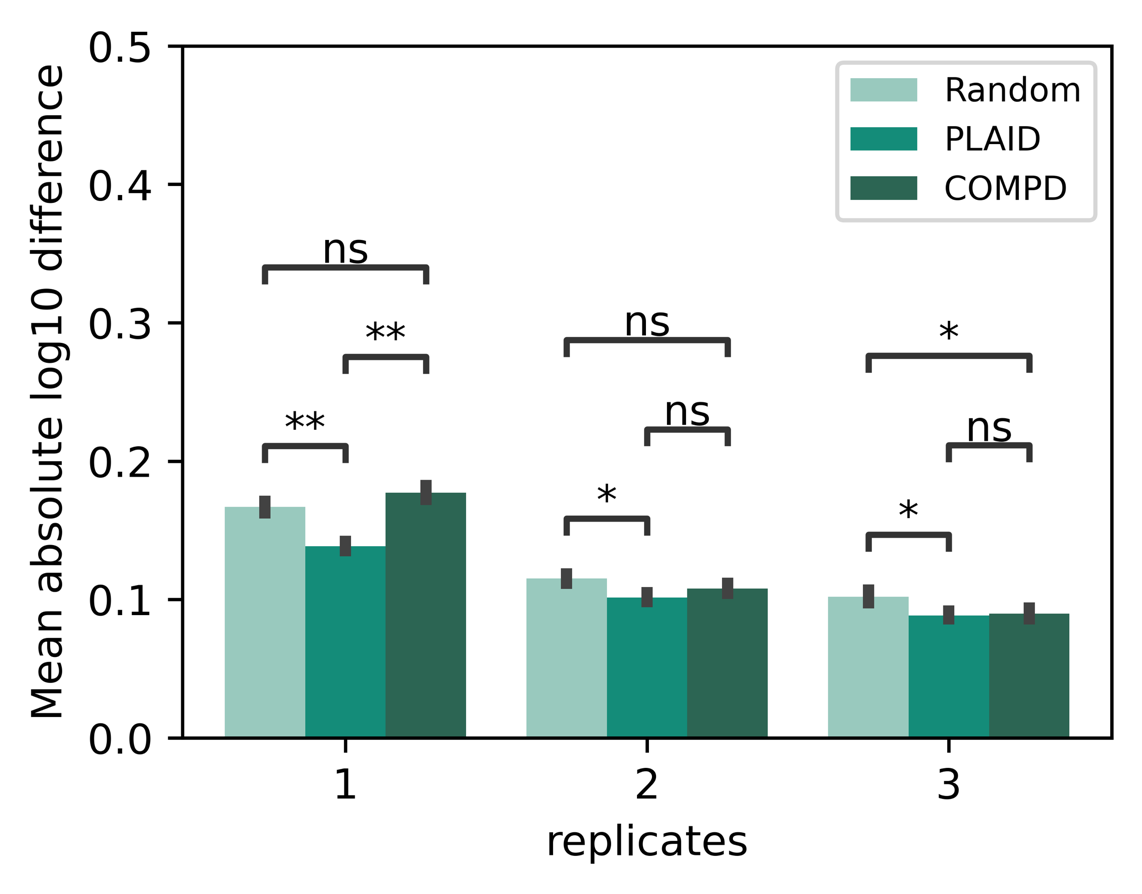
\includegraphics[width=\textwidth]{figures/dose-response-relic50-1-2-3-12doses-dil4-half-columns-neg-controls-0.4.png}
    %\caption{relic50 12doses-dil4-bowl-0.085}
    % \label{fig:tem}
  \end{subfigure}
  \caption{Mean absolute $\log_{10}$ difference between expected and
    obtained values of the relative
    {$\text{EC}_{50}$/$\text{IC}_{50}$} for dose-response curves using
    various numbers of doses, replicates, and plate-effect strengths
    with a linear relationship to column number in the right half of
    the plate. The 4PL sigmoide curves were fitted using compound data
    and 4 negative controls such that their mean was equal to the mean
    of the 20 negative controls the plate. * indicates $p\leq10^{-4}$,
    ** indicates $p\leq10^{-12}$, *** indicates $p\leq10^{-43}$.}
\end{figure*}



%%% Local Variables: 
%%% mode: latex
%%% TeX-master: "supplement.tex"
%%% End: 
